% Description of the leptonic control regions with 4 leptons:
%  - the backgrounds
%  - data/MC plots
%  - table with fake_lepton background yield foreach year

\label{sec:lepCR4l}
Two control regions are defined for the 4\Pl channel with the same requirements as the signal region
except for the selection of one or more leptons, so as to be enriched in \nonprompt and misidentified leptons.
This method was used by several analyses targeting a final state with four leptons from $\PZ\PZ$ decay~\cite{CMS-SMP-16-001, CMS-SMP-17-006, CMS-SMP-20-001, CMS-PAS-SMP-22-001},
and is described in detail in Reference~\cite{CMS-HIG-13-002} as the ``Method using opposite-sign (OS) leptons''.

\paragraph{CR3P1F\\}
In the first region, named CR3P1F, one of the leptons of the $\PZ_2$ must fail the tight selection,
while the other three (both leptons from $\PZ_1$ and the other lepton from $\PZ_2$) must pass the tight identification and isolation criteria.
It is expected to be populated by $\PW\PZ$, with contributions from Drell-Yan and $\PZ\PGg$,
along with a fraction of events from $(\PQq\PAQq/\Pg\Pg) \to \PZ\PZ$ where one of the prompt leptons fails the selection
or falls outside the acceptance and a misidentified jet is reconstructed instead.
Distributions of a few intersting kinematic observables are shown in Figure~\ref{fig:CR3P1F_Run2}.

\begin{figure}
\subfigure [$m_{\PZ_1}$     ] {\includegraphics[width=.333333333\textwidth]{Figures/dataMC_noLFR/Run2/fullMC/CR3P1F/Z0_mass_pow.pdf}}%
\subfigure [$m_{\PZ_2}$     ] {\includegraphics[width=.333333333\textwidth]{Figures/dataMC_noLFR/Run2/fullMC/CR3P1F/Z1_mass_pow.pdf}}%
\subfigure [$m_{\PZ\PZ\PGg}$] {\includegraphics[width=.333333333\textwidth]{Figures/dataMC_noLFR/Run2/fullMC/CR3P1F/ZZG_mass_loosePh_pow.pdf}}
\caption{Invariant mass of the $\PZ_1$, $\PZ_2$ (left and center) without any request on the presence of a photon
  and mass of the $\PZ\PZ\PGg$ system (right) when there is a photon passing the cut-based ID selection,
  in the leptonic control region CR3P1F where one of the leptons from $\PZ_2$ fails the tight selection.}
\label{fig:CR3P1F_Run2}
\end{figure}

\paragraph{CR2P2F\\}
In the second region, named CR2P2F, both leptons from the $\PZ_2$ fail the tight selection, while the leptons of the $\PZ_1$ pass the tight criteria.
This region is populated primarily by Drell-Yan events, with contributions from $\PZ\PGg$ and $\PQt\PAQt+X$.
Some representative distributions for this region are shown in Figure~\ref{fig:CR2P2F_Run2}

\begin{figure}
\subfigure [$m_{\PZ_1}$     ] {\includegraphics[width=.333333333\textwidth]{Figures/dataMC_noLFR/Run2/fullMC/CR2P2F/Z0_mass_pow.pdf}}%
\subfigure [$m_{\PZ_2}$     ] {\includegraphics[width=.333333333\textwidth]{Figures/dataMC_noLFR/Run2/fullMC/CR2P2F/Z1_mass_pow.pdf}}%
\subfigure [$m_{\PZ\PZ\PGg}$] {\includegraphics[width=.333333333\textwidth]{Figures/dataMC_noLFR/Run2/fullMC/CR2P2F/ZZG_mass_loosePh_pow.pdf}}
\caption{Invariant mass of the $\PZ_1$, $\PZ_2$ (left and center) without any request on the presence of a photon
  and mass of the $\PZ\PZ\PGg$ system when there is a photon passing the cut-based ID selection,
  in the leptonic control region CR2P2F where both leptons from $\PZ_2$ fail the tight selection.}
\label{fig:CR2P2F_Run2}
\end{figure}

\paragraph{Contribution to signal region\\}
The expected reducible background in the signal region is given by the sum of two terms:
\begin{itemize}
  \item A 3P1F component, from events with one fake lepton, estimated from the CR3P1F region.
  \item A 2P2F component, from events with two fake leptons, estimated from the CR2P2F region.
\end{itemize}

The 3P1F and 2P2F components are given by the number of events in the respective regions, weighted by factors dependent on the fake rates:
\begin{subequations}
  \begin{align}
    \label{eq:lepFR_3P1Fto4P}
    N^{from\ 3P1F}_{SR} &= \sum_{i \ins 3P1F} \frac{f_a^i}{1-f_a^i}, \quad where\ a = 3, 4
    \\
    \label{eq:lepFR_2P2Fto4P}
    N^{from\ 2P2F}_{SR} &= \sum_{j \ins 2P2F} \frac{f_3^j}{1-f_3^j} \frac{f_4^j}{1-f_4^j}
  \end{align}
\end{subequations}
where $f_3^j$ and $f_4^j$ correspond to the fake rates of the two loose leptons in the j-th event.

However, the CR3P1F region itself has a contribution from fake lepton background events from the CR2P2F region.
These are events with two genuine leptons and two fakes, where only one of the fakes passes the tight selection, thus winding up in the CR3P1F region.
The expected number of background events in the CR3P1F region, $N^{from\ 2P2F}_{3P1F}$,
can be computed from the number of events observed in the CR2P2F control region, $N^{bkg}_{2P2F}$,
by weighting each event in the region with a factor dependent from the fake rates:
\begin{equation}
  \label{eq:lepFR_N3P1F}
  N^{from\ 2P2F}_{3P1F} = \sum_{i \ins 2P2F} \left( \frac{f_i}{1-f_i} + \frac{f_j}{1-f_j} \right)
\end{equation}

Summing all the contributions, one obtains for the signal region:
\begin{equation}
  \begin{split}
    \label{eq:lepFR_4P}
    N^{bkg}_{SR} &= \sum \frac{f^a_i}{1-f^a_i} \left( N_{3P1F} - N^{from\ 2P2F}_{3P1F} \right) + \sum_{j \ins 2P2F} \left( \frac{f_j}{1-f_j} \frac{f_j}{1-f_j} \right)
    \\
                 &= \sum_{i \ins 3P1F} \frac{f^a_i}{1-f^a_i} - \sum_{j \ins 2P2F} \left( \frac{f_j}{1-f_j} \frac{f_j}{1-f_j} \right)
  \end{split}
\end{equation}

More details on the derivation of Equation~\ref{eq:lepFR_4P} can be found in Section~\ref{sec:leptonFR_details}.
